\documentclass{article}
\usepackage[utf8]{inputenc}

\title{Reinforcement Learning- Final Course Project}
\author{Student name (ID. 123456789),Student name ID. 987654321)}
\date{Submitted as final project report for the RL course, BIU, 2024}

\usepackage{natbib}
\usepackage{graphicx}
\usepackage{caption}
\usepackage{subcaption}
\usepackage{xcolor}
\captionsetup[figure]{font={color=gray}}
\usepackage{refstyle}
\usepackage{float}

\begin{document}

\maketitle

\section{Introduction}
This project presents the use of Reinforcement Learning to solve the Sokoban game, a complex puzzle involving the movement of boxes to target locations. We use Deep Q Learning (DQN) for this purpose. This report discusses game design within the context of DQN, analyzes the impact of various hyperparameters on the achieved solutions, and presents successful experiments results.

\section{Solution}
\subsection{General approach}
The Sokoban puzzle presents a grid-based world comprising the agent, walls, boxes, and target locations. The objective is to relocate all boxes to their designated target spots while minimizing the number of actions the agent performs. The agent is capable of executing actions such as moving in any of the four directions (up, down, left, right). The challenge lies in making optimal choices while avoiding dead-ends and loops of futile actions.

DQN represents a model-free reinforcement learning algorithm that operates on reward: this algorithm uses a neural network to approximate the Q-function, which estimates the anticipated cumulative future rewards associated with each possible action within a specific state (Q-values). By instructing the network to approximate these rewards, DQN can establish a policy that maximizes expected rewards over an extended period.

\subsection{Design}
\subsubsection{Network Architecture}
We employ a deep neural network as the function approximating the Q-values. The network  architecture is illustrated in \figref{fig1} and consists of the following components:

\begin{itemize}

\item Input Layer: The input layer represents the current state of the Sokoban puzzle, which is encoded as an RGB picture of the game state.
\item Convolution Layers: Employed for feature extraction.
\item Hidden Layer: A single hidden layer with rectified linear unit (ReLU) activation function.
\item Output Layer: The output layer corresponds to the Q-values for each possible action. It uses a linear activation function.
\end{itemize}

\begin{figure}[H]
  \centering
  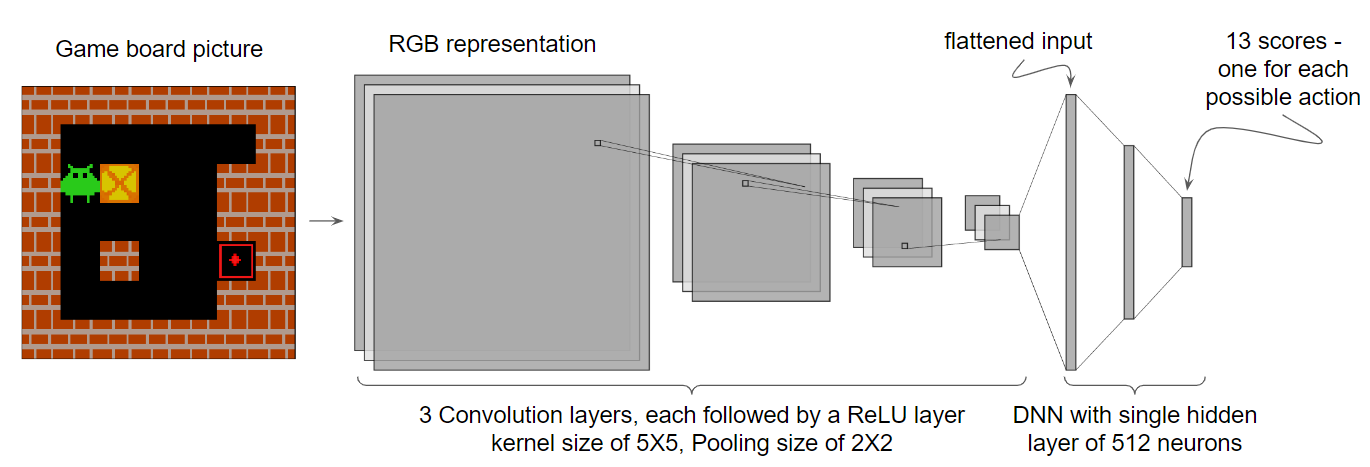
\includegraphics[width=1\columnwidth]{./pics/nework.PNG}
  \caption{Network  architecture illustration}
  \label{fig:fig1}
\end{figure}

\subsubsection{Experience Replay}
Experience replay is the practice of storing an agent's interactions, which include the state, action, reward, and next state, in a dedicated buffer. During the training process, mini-batches of experiences are randomly chosen from this buffer. This reduces the correlation between consecutive experiences during training.

\subsubsection{Target Network}
The target network is a frozen snapshot of the Q-network, and we maintain it this way for a specific number of epochs each time. This prevents the issue of the target Q-values changing too much during training. This improves the stability and convergence of the algorithm.

\section{Experimental results}
To assess the performance of our DQN-based Sokoban solver, we use the following metrics:

\begin{itemize}
\item Episode Length: Average number of steps it takes to solve the Sokoban puzzle, with a maximum limit of 500 steps if the puzzle hasn't been solved by then.
\item Success Rate: The percentage of puzzles successfully solved.
\item Network loss: measures how far off the predicted Q-values are from the actual values. 
\end{itemize}

We measured the metrics during both the training time (for the 500 training episodes) and the testing time (using 10 puzzle samples).
In order to facilitate the exploration of hyperparameters, we will maintain a consistent configuration and systematically vary a single hyperparameter at a time to scrutinize its impact.

\section{Discussion}
Provide some final words and summarize what you have found from running the experiments you described above. Provide some high level insights.

Note - your project will be evaluated for aspects, including the technique you selected, the rational of the experiments you decided to run, the insights you learned from this process and more. Remember, for the purpose of this course, the process that you demonstrate is very  important.

\section{Code}

Please provide a link to your colab notebook.


Good luck!!
\bibliographystyle{plain}
\bibliography{references}
\end{document}
